
%(BEGIN_QUESTION)
% Copyright 2010, Tony R. Kuphaldt, released under the Creative Commons Attribution License (v 1.0)
% This means you may do almost anything with this work of mine, so long as you give me proper credit

Regn ut trykkene $P_1$ and $P_2$, anta at massetettheten til fluidet er 886.45 kg/m³.             

$$\includegraphics[width=15.5cm]{i00457x01.eps}$$

Also, comment on whether or not Bernoulli's equation could be used to compare the suction and discharge pressures of the pump, being that those two pressures (145 and 302 PSI) are measured on the same size pipe, with the same flow rate, and very similar elevations (heights).

\underbar{file i00457}
%(END_QUESTION)





%(BEGIN_ANSWER)

$P_1$ = 296.77 PSI \hskip 30pt $P_2$ = 293.27 PSI

\vskip 10pt

Bernoulli's equation assumes no gain or loss of energy between the two locations compared, and so it {\it cannot} be used to contrast the pump's suction and discharge pressures.  The pump is a machine that adds energy to the fluid going through it, and so the assumption of equal (total) energy between the incoming and outgoing flow streams is not correct.

%(END_ANSWER)





%(BEGIN_NOTES)


%INDEX% Physics, dynamic fluids: Bernoulli's equation

%(END_NOTES)

